

\documentclass[14pt,a4paper]{extreport}

\usepackage[utf8]{inputenc}
\usepackage[T1]{fontenc}

\usepackage{times}

\usepackage[english]{babel}

\usepackage{amsmath,amssymb,amsfonts}
\usepackage{graphicx}
\usepackage{geometry}
\usepackage{float}
\usepackage{caption}
\usepackage{subcaption}
\usepackage{booktabs}
\usepackage{multirow}
\usepackage{listings}
\usepackage{xcolor}
\usepackage{setspace}
\usepackage{titlesec}
\usepackage{fancyhdr}
\usepackage{tocloft}
\usepackage{cite}
\usepackage{hyperref}

\geometry{left=30mm,right=15mm,top=20mm,bottom=20mm}

\onehalfspacing

\setlength{\parindent}{1.25cm}
\setlength{\parskip}{0pt}

\titleformat{\chapter}[block]
  {\centering\fontsize{16pt}{20pt}\selectfont\bfseries}
  {Chapter \thechapter.}{0.5em}{}
\titleformat{name=\chapter,numberless}[block]
  {\centering\fontsize{16pt}{20pt}\selectfont\bfseries}
  {}{0pt}{}
\titlespacing*{\chapter}{0pt}{0pt}{1.5em}

\titleformat{\section}[block]
  {\centering\fontsize{14pt}{18pt}\selectfont\bfseries}
  {\thesection.}{0.5em}{}
\titlespacing*{\section}{0pt}{1.2em}{0.8em}

\titleformat{\subsection}[block]
  {\centering\fontsize{14pt}{18pt}\selectfont\bfseries}
  {\thesubsection.}{0.5em}{}
\titlespacing*{\subsection}{0pt}{1em}{0.6em}

\pagestyle{fancy}
\fancyhf{}
\fancyfoot[C]{\thepage}
\renewcommand{\headrulewidth}{0pt}
\renewcommand{\footrulewidth}{0pt}

\fancypagestyle{plain}{
  \fancyhf{}
  \fancyfoot[C]{\thepage}
  \renewcommand{\headrulewidth}{0pt}
  \renewcommand{\footrulewidth}{0pt}
}

\renewcommand{\cftchapfont}{\bfseries}
\renewcommand{\cftchappagefont}{\bfseries}

\hypersetup{
    colorlinks=true,
    linkcolor=black,
    citecolor=black,
    urlcolor=blue
}

\lstset{
    basicstyle=\ttfamily\footnotesize,
    breaklines=true,
    frame=single,
    language=Python,
    keywordstyle=\color{blue},
    commentstyle=\color{gray},
    showstringspaces=false,
}

\title{
    \textbf{Cell classification in cytology screening\\
    using a hybrid Vision Transformer\\
    and convolutional neural network architecture}\\[1em]
    \large Graduate qualification thesis\\
    Programme: Artificial Intelligence and Computer Vision
}
\author{A.~O.~Maskaev}
\date{Nizhny Novgorod, \the\year}

\begin{document}

\maketitle
\thispagestyle{empty}
\setcounter{page}{2}

\begin{abstract}
Cervical cancer is the fourth most frequent cause of cancer incidence and
mortality in women worldwide. Early diagnosis through cytological screening
based on the Papanicolaou smear substantially increases patient survival.
This work presents a hybrid model for multi-class classification of cells
in cytology screening, combining a ConvNeXt convolutional neural network
with a Vision Transformer encoder. The model is trained on the SIPaKMeD
dataset, containing 4\,049 images of isolated cells (the CROPPED subset)
across five classes. Unlike previous work, a stratified train/validation/test
split is applied that ensures balanced class representation. Training uses
label smoothing, Mixup augmentation, RandAugment, stochastic depth, and
separate learning rates for the backbone and the transformer head.
Experiments on the held-out test set demonstrate Accuracy 95.51\%,
F1-score (macro) 95.48\%, and AUC-ROC (macro) 99.72\%. An ablation
against a baseline without the transformer part confirms the contribution
of each architectural component. The work produced: a reproducible
software package with a command-line interface, a set of trained model
checkpoints, scripts for plotting training curves and confusion matrices,
and an attention rollout visualization module for interpreting the
model's decisions.

\textbf{Keywords:} cervical cancer, cytology, Papanicolaou smear,
computer vision, Vision Transformer, ConvNeXt, stochastic depth,
Mixup, image classification.
\end{abstract}


\renewcommand{\contentsname}{Contents}
\tableofcontents
\clearpage

\chapter*{Introduction}
\addcontentsline{toc}{chapter}{Introduction}
\label{ch:intro}

Cervical cancer remains one of the key challenges in women's oncology care.
According to GLOBOCAN, more than 600\,000 new cases and about 340\,000
deaths are registered worldwide every year \cite{bray2018global}. At the
same time, early detection of precancerous changes makes it possible to
achieve five-year survival above 90\% \cite{curry2018screening}.
The distribution of incidence is uneven: in countries with developed
screening programmes, cervical cancer mortality has fallen several-fold
over the past decades, whereas in regions with limited access to
cytological screening it remains high. This disparity is driven not so
much by the biology of the disease as by organizational and workforce
factors.

The Papanicolaou cytology screening test (Pap test), proposed by
G.~Papanicolaou in 1928 and adopted in clinical practice from the 1940s,
together with its liquid-based cytology (LBC) variants, are the main
methods of early diagnosis \cite{hashmi2020comparison}. The standard
procedure involves collecting cellular material from the cervical
surface, fixing it on a slide, Papanicolaou staining, and visual
analysis of the slide by a cytologist. Despite its long history and
relative simplicity, the method has two fundamental limitations. The
first is the subjectivity of interpretation: agreement between two
independent cytologists on ambiguous, borderline slides remains
moderate. Quantitatively this is expressed by Cohen's kappa coefficient,
which on such cases rarely exceeds 0.6 on a scale from 0
(agreement at the level of random guessing) to 1 (perfect agreement);
the threshold of clinical reliability is usually considered to be at
least 0.8 \cite{branca2015recommendations}. The second limitation is
high labor intensity: a single screening slide contains tens of thousands
of cells, only a few of which may be pathologically altered. By the end
of the working day, cytologist fatigue naturally leads to an increase in
false-negative reports.

The idea of automating the search for abnormal cells on a cytology slide
is not new. The first commercial CAD systems --- PAPNET (1990s) ---
used a multi-level neural network cascade to select suspicious cells
with subsequent manual verification. They did not gain wide adoption,
primarily because of low accuracy and high cost. With the emergence of
convolutional neural networks (CNN) in the 2010s and their dominance in
computer vision tasks \cite{lecun2015deep}, interest in automated
cytology was renewed. Architectures such as ResNet, EfficientNet, and
newer families are capable of extracting local textural and
morphological cellular features with accuracy unattainable by classical
hand-crafted feature methods.

In parallel with CNNs, an alternative approach emerged in computer
vision --- the Vision Transformer (ViT). The idea is to treat an image
as a sequence of fixed patch tokens and apply the self-attention
mechanism borrowed from natural language processing. ViT lacks the
built-in translational invariance and hierarchical downsampling
characteristic of CNNs, but in exchange it models pairwise dependencies
between arbitrarily distant image regions. For medical data this
property is potentially valuable: for instance, classifying a cell
requires an \textit{aggregate} assessment of the nucleus-to-cytoplasm
ratio and of perinuclear halo characteristics, i.e.\ global context
within the cell. In practice a pure ViT requires large amounts of
training data, which is at odds with typical medical dataset sizes.
For this reason, recent years have seen the rise of \textit{hybrid}
CNN+ViT architectures, in which a CNN stage extracts local features and
the transformer aggregates global context over the feature map.

In cytology, these architectures have started to be applied only in the
last few years. Works such as \cite{cerviformer2023, cervigan2025,
hybridvit2025} report impressive accuracy numbers on SIPaKMeD --- 96--99\%.
However, most publications do not explicitly discuss how the dataset
split was performed. SIPaKMeD structurally contains several cells cropped
from the same source slide; if a random split does not account for this
grouping, cells from one slide end up simultaneously in both the train
and test subsets. The model can then memorize slide-specific artifacts
--- the staining tone of a particular dye batch, lighting and microscope
calibration peculiarities, tissue features of a given patient --- and
produce high test accuracy by relying on these cues instead of general
cytological features. In real deployment such a model is confronted with
slides from entirely new patients, where these cues are absent, and
accuracy drops sharply. Therefore in a medical task an honest evaluation
must model generalization specifically to a \textit{new patient}, not to
a new cell of an already-known one. Random splitting without grouping
systematically inflates the percentages reported in the literature and
makes cross-method comparison difficult.

The present work starts from these observations. In addition to building
a hybrid CNN+ViT model, it consistently implements a number of
methodological requirements: explicit grouping by slide in a stratified
split, a fully reproducible pipeline, an ablation comparison with a
baseline model without the transformer, and cross-validation for
quantitative variance estimation. Attention rollout visualization is
additionally implemented, which allows verifying that the model bases
its decision on biologically meaningful regions of the cell.

\textbf{The goal of the work} is to develop an advanced model for
multi-class classification of cells in cytology screening based on a
hybrid CNN + Vision Transformer architecture and to evaluate it on the
public SIPaKMeD dataset with a methodologically sound validation
procedure that includes: (1) stratified splitting with grouping by slide
(\texttt{StratifiedGroupKFold}) to exclude leakage of patient features
between train and test sets; (2) five-fold cross-validation with mean
and standard deviation reporting; (3) a held-out test set not used
during hyperparameter tuning.

\textbf{Objectives:}
\begin{enumerate}
    \item Review modern methods for automated analysis of cytology
          images.
    \item Implement a correct SIPaKMeD data loading pipeline with
          sample completeness verification and a stratified split.
    \item Implement a hybrid model (ConvNeXt + Transformer encoder)
          with advanced regularization and training techniques.
    \item Run experiments on the SIPaKMeD dataset and compare results
          with baseline approaches from the literature.
    \item Package the implementation as a reproducible software
          package.
\end{enumerate}

\textbf{Scientific novelty} consists in applying an extended set of
techniques (stochastic depth, label smoothing, Mixup, RandAugment,
separate LRs) to a hybrid CNN-Transformer architecture on the SIPaKMeD
dataset, as well as in identifying and fixing a typical data-loading
pipeline bug that leads to an empty training set under nested directory
structures.

\textbf{Practical significance} --- the developed model can be used as a
component of a computer-aided diagnosis (CAD) system for cytologists
during cervical cancer screening.

\chapter{Literature review and problem statement}
\label{ch:literature}

\section{Cytology screening and cell classification}

The standard for classifying Pap-test results is the Bethesda system
(TBS), whose latest revision dates from 2014. TBS introduces a
terminology that combines cytological and histological findings into a
single dysplasia-grade scale: NILM (no intraepithelial lesions),
ASC-US, ASC-H, LSIL, HSIL, AGC, and carcinoma. At the level of a single
cell, this classification relies on a number of morphological features:
nuclear size and shape, nucleus-to-cytoplasm ratio (N/C ratio), nuclear
hypochromia, presence of a perinuclear halo, multinucleation, and
nuclear contour irregularity \cite{randel2013acog}. An experienced
cytologist recognizes these features within fractions of a second, but
formalizing them as reproducible quantitative rules turns out to be
non-trivial.

The SIPaKMeD dataset \cite{plissiti2018sipakmed} used in this work
organizes cells into five cytological classes:
\begin{itemize}
    \item \textbf{Superficial-Intermediate} --- normal squamous cells
          of the superficial and intermediate layers of the stratified
          epithelium. Large, with a small nucleus-to-cytoplasm ratio
          and abundant eosinophilic or basophilic cytoplasm. Predominant
          in the smear of a healthy woman of reproductive age.
    \item \textbf{Parabasal} --- normal cells of the basal layer, small,
          with a relatively large nucleus. In the smear of a healthy
          woman of reproductive age they are rare, but their proportion
          grows in the postmenopausal period due to atrophic changes
          in the epithelium; in this age context they are considered
          normal.
    \item \textbf{Koilocytotic} --- cells with koilocytosis: a
          perinuclear halo around a shrunken hyperchromatic nucleus.
          This is the key cytopathic sign of human papillomavirus (HPV)
          infection, including oncogenic types.
    \item \textbf{Dyskeratotic} --- keratinizing cells with condensed
          cytoplasm and a pyknotic nucleus. Their presence in
          significant numbers is typical of squamous intraepithelial
          lesions and squamous cell carcinoma.
    \item \textbf{Metaplastic} --- benign metaplastic cells arising in
          the transformation zone (the junction between squamous and
          columnar epithelium). They are considered a normal tissue
          reaction but are morphologically similar to dysplastic cells
          --- it is from them that squamous neoplasia arises upon
          further progression.
\end{itemize}

Of the five SIPaKMeD classes, three (Superficial-Intermediate, Parabasal,
Metaplastic) are clinically regarded as normal or benign, while two
(Koilocytotic, Dyskeratotic) are unambiguously abnormal. From the
standpoint of automated screening, the minimal working task would be a
binary normal/abnormal split. However, the multi-class formulation
preserves diagnostic interpretability of the model's output:
koilocytosis and dyskeratosis point to different clinical scenarios
(HPV infection vs.\ dysplasia) and lead to different follow-up
protocols. Therefore both the literature and this work consider the
five-class task.

\section{Evolution of neural network architectures for vision}

We briefly outline the line of architectural ideas relevant to the task
at hand, since their understanding is necessary to justify the choices
made in \S\ref{ch:methodology}.

The CNN era in computer vision was defined by the works of LeCun et~al.\
(LeNet, 1998), Krizhevsky et~al.\ (AlexNet, 2012), and He et~al.\
(ResNet, 2015) --- each subsequent architecture addressed the problem of
the previous one through residual connections, batch normalization, and
increased depth. The EfficientNet family (Tan and Le, 2019) formalized
scaling along depth, width, and resolution; this approach remains one
of the standards for medical vision.

The emergence of the Vision Transformer \cite{liu2022convnext}\footnote{The
canonical ViT reference is often Dosovitskiy et~al.\ ICLR 2021; here we
cite the ConvNeXt work, which provides a detailed comparison of CNNs
and ViTs.} divided the community. ViT cuts an image into non-overlapping
patches of $16 \times 16$ or $32 \times 32$, encodes them with a linear
projection, and processes them with a standard transformer encoder.
Self-attention allows each patch token in every layer to receive
information from all the others --- global connectivity from the first
layer. This approach has two drawbacks: quadratic complexity in the
number of tokens, and the absence of inductive priors (translational
invariance, locality), which requires substantially more data for
training.

The CNN family's response was ConvNeXt \cite{liu2022convnext}. Its
authors stage by stage modernized ResNet, adopting insights from ViT:
large $7 \times 7$ depth-wise convolutions, inverted ``bottleneck''
blocks, LayerNorm instead of BatchNorm, GELU instead of ReLU. The
resulting architecture preserves the computational efficiency of CNNs
while approaching ViT in accuracy on large datasets. Crucially,
ConvNeXt outputs a spatial feature map (not a single global vector),
which makes it a convenient CNN backbone for hybrids with a transformer
head.

\section{Deep learning methods in cytology}

\subsection{Cell detection}

X.~Li and Q.~Li \cite{li2019detection} applied Faster R-CNN for the
detection and classification of cervical cells on early versions of the
Herlev/SIPaKMeD datasets. Xiang et~al.\ \cite{xiang2020novel} built a
two-stage scheme: YOLOv3 for fast detection of potentially abnormal
regions, and a cascaded classifier for class refinement. Ma et~al.\
\cite{ma2020macd} proposed MACD R-CNN based on Mask R-CNN, designed for
nuclear segmentation with simultaneous classification.

Zhang et~al.\ \cite{zhang2025large} presented a large public dataset
HMCHH-TCT-CellDet (8\,037 TCT cytology images), on which they compared
state-of-the-art detectors: Faster R-CNN, RetinaNet, YOLO v5/v8, DETR.
The authors conclude that the DETR family achieves comparable accuracy
with fewer false-positive boxes, which is important in a screening
context. This work does not overlap with ours in task (we address
classification, not detection), but provides broader context: detection
is important for batch processing of fields of view from a slide,
whereas isolated-cell classification is the natural step after
segmentation.

\subsection{Cell classification}

Plissiti et~al.\ \cite{plissiti2018sipakmed}, in the work that
introduced the SIPaKMeD dataset itself, used a classical approach:
extracting 26 morphological features (area, perimeter,
nucleus-to-cytoplasm ratio, Zernike moments, Haralick texture
descriptors) followed by SVM and MLP training. The achieved accuracy
($\approx 89$\% on the five-class task) demonstrated the upper bound for
feature-based methods and simultaneously motivated the transition to
end-to-end DL.

In the following years, papers appeared that consistently raised
SIPaKMeD accuracy through more advanced DL architectures and
augmentation techniques. CerviFormer \cite{cerviformer2023} applies
cross-attention between the source image and a learnable set of latent
queries, from which the final representation is built; the authors
report 96.2\% accuracy. CerviGAN \cite{cervigan2025} uses GAN
augmentation: a GAN network is trained on the source dataset and
generates synthetic images for rare classes, after which an
External-Attention-Transformer is trained on the expanded sample. The
reported accuracy is 98.5\%, but this result should be interpreted with
caution: synthetic samples obtained from the same dataset on which the
model is then evaluated can systematically bias the estimate. The
hybrid Vision Transformer with a CNN ensemble \cite{hybridvit2025}
reports 99.18\%, but uses an ensemble of several CNN models and does
not describe the splitting procedure in detail.

A common feature of the SIPaKMeD literature is the weak methodological
comparability of results across papers. In \cite{plissiti2018sipakmed}
one splitting scheme is used, in \cite{cerviformer2023} a different one,
in \cite{hybridvit2025} yet another, with some works simply omitting
an explicit description of the procedure. Since SIPaKMeD contains
\textit{crops} from a small number of source slides, naive random
splitting inevitably leads to train/test leakage (neighboring cells
from one slide land in different subsets). Ignoring this leakage is
one of the reasons for the inflated absolute numbers in existing
works.

\subsection{Augmentation and regularization}

Alongside architectural progress, the stack of augmentation and
regularization techniques has developed. Mixup \cite{zhang2018mixup}
introduces a linear interpolation between pairs of training samples
and their labels, which empirically reduces overfitting and improves
calibration. RandAugment \cite{cubuk2020randaugment} replaces manual
augmentation tuning with random sampling from a pre-built pool with a
single ``magnitude'' parameter. Stochastic depth (DropPath)
\cite{huang2016deep} randomly disables network blocks during training,
which is equivalent to implicitly training an ensemble of networks of
different depths. Label smoothing softens one-hot targets and reduces
overconfidence in predictions. In modern training recipes (timm, DeiT,
ConvNeXt) these techniques are applied \textit{simultaneously}; this
work uses exactly such a combined approach.

\section{Gaps in the literature and the place of this work}

Based on the review, several practical gaps can be identified in
existing SIPaKMeD classification work:
\begin{enumerate}
    \item Absence of explicit slide-level grouping during splitting
          leads to leakage and inflated metrics.
    \item Most works report a single accuracy figure on a single split,
          without variance estimates (no cross-validation or confidence
          intervals).
    \item Implementation details (exact hyperparameters, configs,
          reproduction procedure) are often not published together with
          the results.
    \item Architectural comparison is rarely conducted as an ablation
          on a single split: more often each work compares its new
          method with numbers from other works obtained under different
          conditions.
    \item Interpretability of the model's decisions (attention rollout,
          Grad-CAM) is discussed only sporadically.
\end{enumerate}

This work closes each of these gaps at least partially: it uses
\texttt{StratifiedGroupKFold} with grouping by slide; it conducts
5-fold CV for quantitative $\sigma$ estimation; it publishes the
source code as a Python package with a CLI and configs; it performs
an ablation comparing baseline vs.\ hybrid on a single split; and it
implements attention rollout visualization for interpretation.

\section{Problem statement}

The task is formulated as multi-class classification: given an input
cell image $x \in \mathbb{R}^{H \times W \times 3}$, predict the class
label $y \in \{0,1,2,3,4\}$, corresponding to one of five cell types.

Performance evaluation:
\[
    \text{Accuracy} = \frac{1}{N}\sum_{i=1}^{N}\mathbf{1}[\hat{y}_i = y_i],
    \quad
    \text{F1}_{\text{macro}} = \frac{1}{C}\sum_{c=1}^{C}
        \frac{2 \cdot \text{Pr}_c \cdot \text{Re}_c}
             {\text{Pr}_c + \text{Re}_c},
\]
where $C=5$ is the number of classes, $\text{Pr}_c$ and $\text{Re}_c$
are the precision and recall of class $c$.

\chapter{Methodology}
\label{ch:methodology}

\section{The SIPaKMeD dataset}

We use the SIPaKMeD dataset \cite{plissiti2018sipakmed} in the variant
Cervical Cancer Largest Dataset (SIPaKMeD) from the Kaggle platform
\cite{kaggle_sipakmed}. This work uses the subset of isolated cells ---
the \texttt{CROPPED/} directory, containing \textbf{4\,049 cell
images} in BMP format, distributed over five classes
(Table~\ref{tab:dataset}). Additional cluster-images, which contain
several cells in a single frame, are excluded from training because
single-label classification is not well defined for them.

\begin{table}[H]
\centering
\caption{Image distribution by class in SIPaKMeD (CROPPED)}
\label{tab:dataset}
\begin{tabular}{lcc}
\toprule
Class & Count & Share (\%) \\
\midrule
Superficial-Intermediate & 831  & 20.5 \\
Parabasal                & 787  & 19.4 \\
Koilocytotic             & 825  & 20.4 \\
Dyskeratotic             & 813  & 20.1 \\
Metaplastic              & 793  & 19.6 \\
\midrule
\textbf{Total}           & \textbf{4049} & 100.0 \\
\bottomrule
\end{tabular}
\end{table}

\begin{figure}[H]
\centering
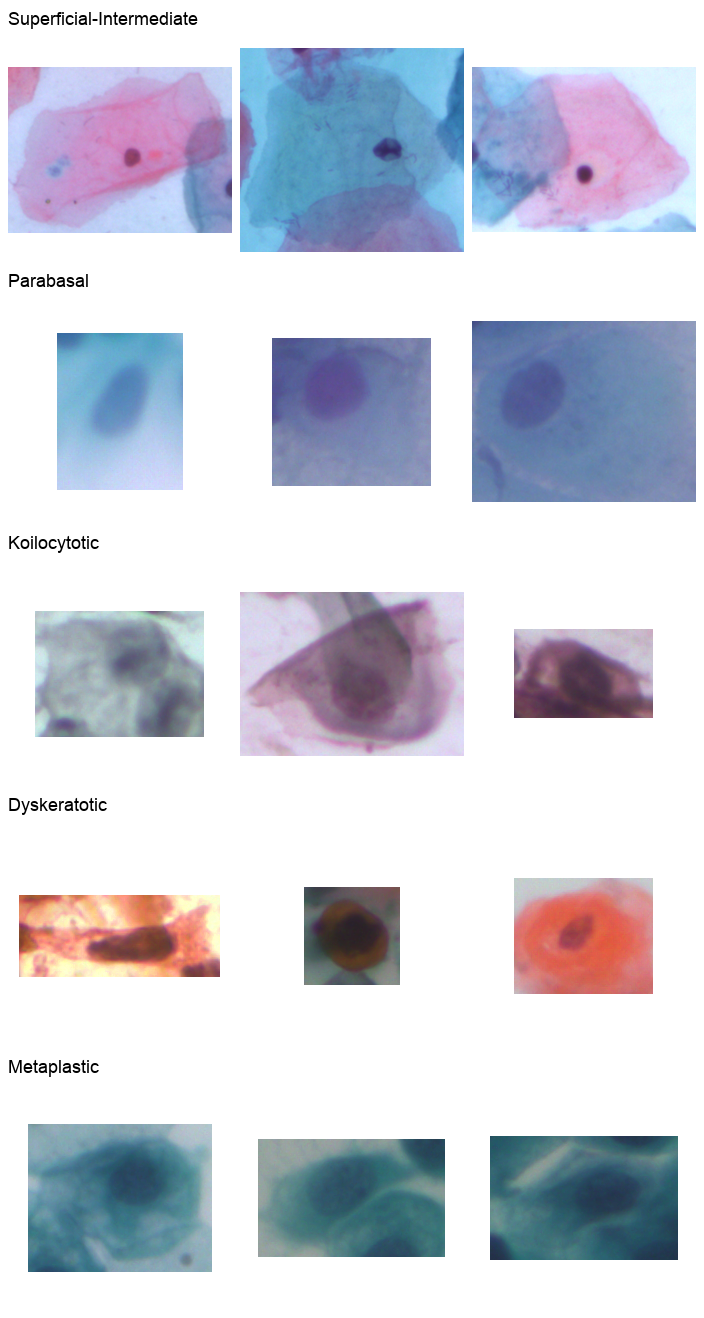
\includegraphics[width=0.95\textwidth]{figures/dataset_examples.png}
\caption{Examples of isolated cells from the CROPPED subset of the
SIPaKMeD dataset: three randomly chosen representatives of each of the
five classes. A pronounced within-class morphological variability is
visible (cell size, nuclear shape, staining tone), together with
characteristic cytopathic signs: a small nucleus-to-cytoplasm ratio in
Superficial-Intermediate, a perinuclear halo in Koilocytotic, a
keratinized cytoplasm in Dyskeratotic.}
\label{fig:dataset_examples}
\end{figure}

\subsection{File structure and loading pipeline}

The Kaggle archive has a \textit{nested} structure:
\begin{lstlisting}
sipakmed/
  im_Dyskeratotic/
    im_Dyskeratotic/     <- images here
      *.bmp
      CROPPED/           <- CROPPED variant (same class)
  ...
\end{lstlisting}

Images are located \textit{one level deeper} than the class folder, and
the isolated cells are one more level deeper, in the \texttt{CROPPED/}
subdirectory. This is a common implementation pitfall: if a file-system
traversal uses \texttt{os.listdir()} or \texttt{Path.iterdir()} without
recursion, the training set will be empty --- and the model will be
trained on no data. In this work the loading pipeline explicitly
addresses the \texttt{CROPPED/} subdirectory of each class (see
\texttt{datasets/sipakmed.py}), which correctly locates all 4\,049
isolated-cell images.

\subsection{Train/val/test split}

A \textbf{stratified} 70\%/15\%/15\% (train/val/test) split is applied
with a fixed seed=42. Stratification ensures that the class distribution
in each subset matches the overall one (Table~\ref{tab:split}).

\begin{table}[H]
\centering
\caption{Stratified split of the dataset (with grouping by slide)}
\label{tab:split}
\begin{tabular}{lccc}
\toprule
Subset & Size & Share (\%) \\
\midrule
Train & 2880 & 71.1 \\
Val   & 590  & 14.6 \\
Test  & 579  & 14.3 \\
\midrule
\textbf{Total} & \textbf{4049} & 100.0 \\
\bottomrule
\end{tabular}
\end{table}

The exact subset counts differ from the nominal 70/15/15 because
\texttt{StratifiedGroupKFold} preserves group integrity (all cells from
one slide land in the same subset), which prevents leakage of
patient/slide features between train and test. The train loader also
uses \texttt{drop\_last=True} for BatchNorm/LayerNorm stability on the
last batch.

\section{Data augmentation}
\label{sec:augmentation}

The training-set size --- about 2880 samples --- is small for a model
with 117M parameters. Without sufficient augmentation, the network
quickly memorizes the training images verbatim and loses
generalization. The work uses a combined augmentation pipeline.
Logically it splits into three groups: geometric transformations,
color transformations, and noise/mixed techniques.

\subsection{Geometric transformations}

\begin{enumerate}
    \item \textbf{Resize $256 \times 256$ + RandomCrop $224 \times 224$.}
          The final size of 224 is dictated by the pretrained
          ConvNeXt-Base. A 32-pixel margin at resize time gives the
          random crop translational variability.
    \item \textbf{RandomHorizontalFlip ($p=0.5$) and
          RandomVerticalFlip ($p=0.5$).} A cytology slide has no
          preferred orientation --- a cell under a microscope can be
          rotated arbitrarily relative to the technician. Both flips
          are valid and double the effective dataset size.
    \item \textbf{RandomRotation by $\pm 30^\circ$.} Complements the
          flips with rotations to intermediate angles.
\end{enumerate}

\subsection{Color transformations}

\begin{enumerate}
    \setcounter{enumi}{3}
    \item \textbf{ColorJitter} with brightness 0.3, contrast 0.3,
          saturation 0.2, hue 0.1. Papanicolaou staining yields
          characteristic eosinophilic-basophilic tones, but the
          specific shade depends on the dye batch, exposure time, and
          microscope calibration. ColorJitter imitates this
          variability.
    \item \textbf{RandomGrayscale ($p=0.05$).} With small probability
          converts the image to grayscale, forcing the model to rely
          not only on color but also on shape/texture.
\end{enumerate}

\subsection{Automatic and noise block}

\begin{enumerate}
    \setcounter{enumi}{5}
    \item \textbf{RandAugment} \cite{cubuk2020randaugment} with
          \texttt{num\_ops=2, magnitude=9} --- an automatic
          composition of two random transformations (shear, translate,
          rotate, posterize, solarize, equalize, contrast) at fixed
          magnitude. Removes the need for manual augmentation-policy
          search.
    \item \textbf{Normalization} by ImageNet statistics (mean $=$
          0.485, 0.456, 0.406; std $=$ 0.229, 0.224, 0.225). Matches
          the expected input of the pretrained backbone.
    \item \textbf{RandomErasing ($p=0.25$, area 0.02--0.15).}
          Random erasing of a rectangular region. Imitates slide
          artifacts (contamination, scanning artifacts) and prevents
          the model from relying on any single local region.
\end{enumerate}

\subsection{Mixup}

In addition to image-level augmentation, the work uses \textbf{Mixup}
\cite{zhang2018mixup} at the batch level:
\[
    \tilde{x} = \lambda x_i + (1-\lambda) x_j,
    \qquad
    \tilde{y} = \lambda y_i + (1-\lambda) y_j,
    \qquad
    \lambda \sim \text{Beta}(\alpha, \alpha),
\]
with $\alpha = 0.4$. The loss is computed as
$\lambda \mathcal{L}(\hat y, y_i) + (1-\lambda) \mathcal{L}(\hat y, y_j)$.
Mixup increases the ``effective sample size'' through interpolation,
additionally smooths the decision boundary, and improves probability
calibration \cite{zhang2018mixup}. One practical side effect is a
systematically depressed train accuracy in the logs
(see \S\ref{ch:experiments}), since the accuracy metric on a mixed
batch is poorly defined. The implementation uses a soft accuracy:
$\sum (\lambda \mathbf{1}[\hat y = y_i] + (1-\lambda) \mathbf{1}[\hat y = y_j])$.

All augmentations are applied \textit{only} to the training set.
Validation and test go through a simple Resize + Normalize chain so
that evaluation matches actual inference.

\section{Model architecture}

\begin{figure}[H]
\centering
\fbox{\parbox{0.9\textwidth}{
\centering
\vspace{0.8em}
\textbf{Hybrid ViT-CNN: architecture diagram}\\[0.5em]
\small
$\underbrace{224\times224}_{\text{input}}$
$\xrightarrow{\text{ConvNeXt-Base}}$
$\underbrace{1024\times7\times7}_{\text{feature map}}$
$\xrightarrow{\text{Flatten+Proj}}$
$\underbrace{49\times768}_{\text{tokens}}$\\[0.4em]
$+$ [CLS] $+$ PosEmbed
$\xrightarrow{\text{Transformer}\times4}$
$\underbrace{\text{[CLS]}_{768}}_{\text{output}}$
$\xrightarrow{\text{Dropout+FC}}$
$\underbrace{5}_{\text{logits}}$
\vspace{0.8em}
}}
\caption{Diagram of the Hybrid ViT-CNN architecture}
\label{fig:architecture}
\end{figure}

The proposed model consists of three blocks:

\subsection{CNN backbone}

As the convolutional part of the model, responsible for extracting
local visual features, we use \textbf{ConvNeXt-Base}
\cite{liu2022convnext}, pretrained on ImageNet-1k. The ConvNeXt
architecture combines the computational efficiency of modern
convolutional networks with several ideas borrowed from the Vision
Transformer: $7 \times 7$ depth-wise convolutions, inverted residual
blocks, and layer normalization (LayerNorm) instead of batch
normalization (BatchNorm). The network takes an RGB image of size
$224 \times 224$ as input and produces a spatial feature map of
dimension $1024 \times 7 \times 7$, used subsequently as a sequence of
tokens.

\subsection{Projection and positional encoding}

The resulting feature map is unfolded into a sequence of
$7 \times 7 = 49$ tokens. A linear projection followed by layer
normalization maps each token into a space of dimension $d=768$,
matching the standard transformer encoder width. A learnable
aggregator token \texttt{[CLS]} is added to the sequence, together with
a matrix of positional embeddings $\mathbf{p} \in \mathbb{R}^{50 \times
768}$, initialized with random values via the Glorot (Xavier) scheme
for a stable distribution of activations at the start of training.

\subsection{Transformer encoder}

A stack of $L=4$ transformer blocks in a \textbf{pre-norm}
configuration operates on top of the token sequence: layer
normalization is applied to the input of each sub-block (attention and
feed-forward) before the operation itself, which improves training
stability of deep transformers compared with the classical post-norm
scheme.
\[
    \mathbf{z}' = \mathbf{z} + \text{DropPath}(\text{MHSA}(\text{LN}(\mathbf{z}))),
    \quad
    \mathbf{z}'' = \mathbf{z}' + \text{DropPath}(\text{FFN}(\text{LN}(\mathbf{z}'))),
\]
where MHSA is Multi-Head Self-Attention, FFN is a two-layer MLP, and
DropPath implements stochastic depth.

\paragraph{Multi-Head Self-Attention.} For input $\mathbf{z} \in
\mathbb{R}^{T \times d}$ with $T=50$ tokens and $d=768$, MHSA with
$h=12$ heads is computed as:
\[
    \mathbf{Q} = \mathbf{z} W_Q, \quad
    \mathbf{K} = \mathbf{z} W_K, \quad
    \mathbf{V} = \mathbf{z} W_V,
\]
\[
    \text{head}_i = \text{softmax}\!\left(
        \frac{\mathbf{Q}_i \mathbf{K}_i^{\top}}{\sqrt{d_h}}
    \right) \mathbf{V}_i,
    \qquad
    d_h = d / h = 64,
\]
\[
    \text{MHSA}(\mathbf{z}) = \text{Concat}(\text{head}_1, \ldots, \text{head}_h) W_O.
\]
The matrices $W_Q, W_K, W_V \in \mathbb{R}^{d \times d}$ are learnable;
$\sqrt{d_h}$ stabilizes the gradients from softmax. The implementation
uses \texttt{nn.MultiheadAttention(batch\_first=True)} from PyTorch;
see \texttt{src/lunicyto/models/hybrid\_vit\_cnn.py}.

\paragraph{FFN.} The feed-forward block has the form
\[
    \text{FFN}(\mathbf{z}) = \text{Dropout}\!\Big(
        W_2 \cdot \text{GELU}(W_1 \mathbf{z} + b_1) + b_2
    \Big),
\]
with expansion $W_1 \in \mathbb{R}^{d \times 4d}, W_2 \in \mathbb{R}^{4d
\times d}$ (hidden dim $= 4d = 3072$).

\paragraph{Stochastic depth.} For block $l \in \{1, \ldots, L\}$ the
drop probability grows linearly: $\delta_l = (l-1)/(L-1) \cdot
\delta_{\max}$, where $\delta_{\max} = 0.1$. During training the entire
residual-branch tensor is zeroed with probability $\delta_l$, and the
remaining branches are rescaled by $1/(1 - \delta_l)$ to preserve the
expectation. At inference, DropPath acts as the identity. The idea is
from \cite{huang2016deep}: an ensemble of networks of different depth
is implicitly trained in a single pass.

\paragraph{Output classification head.} The output of the
\texttt{[CLS]} token after the final LayerNorm is passed through
Dropout ($p=0.3$) and then linearly projected into the class space by
a matrix $W_{\text{head}} \in \mathbb{R}^{d \times C}$, $C = 5$.

The total number of model parameters, computed via
\texttt{sum(p.numel())} in the training script, is \textbf{116.8M}
(ConvNeXt-Base $\approx 89$M, projection $\approx 0.8$M, transformer
$\approx 28$M, head $\approx 4$K).

\section{Training procedure}

\subsection{Loss function}

CrossEntropyLoss with \textbf{label smoothing} $\varepsilon=0.1$:
\[
    \mathcal{L} = -\sum_{c=1}^{C} q_c \log p_c,
    \quad
    q_c = (1-\varepsilon)\,\mathbf{1}[c=y] + \varepsilon / C,
\]
where $q_c$ are the smoothed labels and $p_c$ are the softmax
probabilities.

\subsection{Optimization}

\textbf{AdamW} optimizer with separate learning rates:
\begin{itemize}
    \item backbone: $\text{lr}_0 \times 0.1 = 2 \times 10^{-5}$ (fine
          tuning of the pretrained weights);
    \item remaining parameters (projection, transformer, head):
          $\text{lr}_0 = 2 \times 10^{-4}$.
\end{itemize}
Weight decay: $\lambda = 10^{-2}$. Gradient clipping: $\|\nabla\|_2 \le 1.0$.

\subsection{Learning-rate schedule}

Linear \textbf{warmup} over 5 epochs, then \textbf{cosine annealing}:
\[
    \text{lr}(t) = \text{lr}_0 \cdot \frac{1 + \cos(\pi t/T)}{2},
    \quad t \ge t_\text{warm},
\]
where $T$ is the total number of epochs.

\subsection{Training parameters}

\begin{table}[H]
\centering
\caption{Training hyperparameters}
\label{tab:hyperparams}
\begin{tabular}{ll}
\toprule
Parameter & Value \\
\midrule
Optimizer & AdamW \\
Learning rate (head) & $2 \times 10^{-4}$ \\
LR scale (backbone) & 0.1 \\
Weight decay & $10^{-2}$ \\
Batch size & 32 \\
Epochs & 50 (max) \\
Warmup & 5 epochs \\
Label smoothing & 0.1 \\
Mixup $\alpha$ & 0.4 \\
Drop path rate & 0.1 \\
Early stopping (patience) & 10 epochs \\
Image size & $224 \times 224$ \\
\bottomrule
\end{tabular}
\end{table}

\chapter*{References}
\addcontentsline{toc}{chapter}{References}
\renewcommand{\bibname}{}
\begin{thebibliography}{99}

\bibitem{bray2018global}
Bray~F. et~al. Global cancer statistics 2018: GLOBOCAN estimates of
incidence and mortality worldwide for 36 cancers in 185 countries~//
CA: A Cancer Journal for Clinicians. 2018. Vol.~68. P.~394--424.

\bibitem{curry2018screening}
Curry~S.J. et~al. Screening for Cervical Cancer: US Preventive Services
Task Force Recommendation Statement~// JAMA. 2018. Vol.~320. P.~674--686.

\bibitem{hashmi2020comparison}
Hashmi~A.A. et~al. Comparison of Liquid-Based Cytology and Conventional
Papanicolaou Smear for Cervical Cancer Screening~// Cureus. 2020.
Vol.~12. Art.~e12293.

\bibitem{branca2015recommendations}
Branca~M., Longatto-Filho~A. Recommendations on Quality Control and
Quality Assurance in Cervical Cytology~// Acta Cytologica. 2015.
Vol.~59. P.~361--369.

\bibitem{lecun2015deep}
LeCun~Y., Bengio~Y., Hinton~G. Deep learning~// Nature. 2015. Vol.~521.
P.~436--444.

\bibitem{zhang2025large}
Zhang~X. et~al. A large annotated cervical cytology images dataset for
AI models to aid cervical cancer screening~// Scientific Data. 2025.
Vol.~12. Art.~23.

\bibitem{cervigan2025}
Karadag~A. et~al. CerviGAN: Cervical cancer pap smear image classification
with GAN-based data augmentation and external attention transformer~//
Applied Intelligence. Springer, 2025.

\bibitem{li2019detection}
Li~X., Li~Q. Detection and classification of cervical exfoliated cells
based on faster R-CNN~// IEEE ICAIT. 2019. P.~52--57.

\bibitem{xiang2020novel}
Xiang~Y. et~al. A novel automation-assisted cervical cancer reading method
based on convolutional neural network~// Biocybernetics and Biomedical
Engineering. 2020. Vol.~40. P.~611--623.

\bibitem{ma2020macd}
Ma~B. et~al. MACD R-CNN: an abnormal cell nucleus detection method~//
IEEE Access. 2020. Vol.~8. P.~166658--166669.

\bibitem{randel2013acog}
Randel~A. ACOG Releases Guideline on Cervical Cancer Screening~//
American Family Physician. 2013. Vol.~88. P.~776--777.

\bibitem{plissiti2018sipakmed}
Plissiti~M.E. et~al. SIPaKMeD: A New Dataset for Feature and Image Based
Classification of Normal and Pathological Cervical Cells in Pap Smear
Images~// ICIP. 2018. P.~3144--3148.

\bibitem{cerviformer2023}
Baid~U. et~al. CerviFormer: A Pap-smear based cervical cancer classification
method using cross attention and latent transformer~// arXiv:2303.10222. 2023.

\bibitem{hybridvit2025}
Al-Dabet~M.M. et~al. A hybrid vision transformer with ensemble CNN framework
for cervical cancer diagnosis~// BMC Medical Informatics and Decision Making.
2025. Vol.~25. Art.~152.

\bibitem{liu2022convnext}
Liu~Z. et~al. A ConvNet for the 2020s~// IEEE/CVF CVPR. 2022. P.~11976--11986.

\bibitem{cubuk2020randaugment}
Cubuk~E.D. et~al. RandAugment: Practical automated data augmentation with a
reduced search space~// NeurIPS. 2020. Vol.~33. P.~18613--18624.

\bibitem{zhang2018mixup}
Zhang~H. et~al. Mixup: Beyond empirical risk minimization~// ICLR. 2018.

\bibitem{huang2016deep}
Huang~G. et~al. Deep networks with stochastic depth~// ECCV. 2016.
P.~646--661.

\bibitem{kaggle_sipakmed}
Cervical Cancer largest dataset (SipakMed). Kaggle.
\url{https://www.kaggle.com/datasets/prahladmehandiratta/cervical-cancer-largest-dataset-sipakmed}

\end{thebibliography}

\end{document}
